\documentclass[11pt,aps,prb,groupedaddress,nofootinbib,floatfix]{beamer}
\usetheme{Goettingen}

\addtobeamertemplate{navigation symbols}{}{%
    \usebeamerfont{footline}%
    \usebeamercolor[fg]{footline}%
    \hspace{1em}%
    \insertframenumber/\inserttotalframenumber
}

%\usepackage[utf8]{inputenc}
\usepackage{amsmath}
\usepackage{amsfonts}
\usepackage{amssymb}
\usepackage{graphicx}
\usepackage[absolute,overlay]{textpos}
\usepackage{chronology}
\usepackage{tikz}
\usepackage{hyperref}
\usepackage{listings}
\usepackage{cite}
\newcommand{\pollaroid}{\emph{Poll}aroid}
\newcommand{\code}{\texttt}
\newcommand\blankfootnote[1]{%
  \let\thefootnote\relax\footnotetext{#1}%
  \let\thefootnote\svthefootnote%
}
\author{Harlan Haskins\\Joshua Robbins\\Stuart Olivera\\Luke Shadler}
\title{\pollaroid : Polling for the People!}
%\setbeamercovered{transparent} 
%\setbeamertemplate{navigation symbols}{} 
%\logo{} 
\institute{Rochester Institute of Technology} 
%\date{} 
%\subject{} 
\begin{document}

\begin{frame}
\titlepage
\end{frame}


\section{Motivation}


%
%	A Need for a better Polling source
%
\begin{frame}{Being Polled Sucks}
\begin{itemize}
	\item Untimely or unwanted calls
	\item Voicing an opinion to a representative is lost in cyberspace
	\item Politicians are notorious from hiding viewpoints
\end{itemize}
\end{frame}

%
%   Pollaroid!
%
\begin{frame}{Introducing...\pollaroid!}
\begin{itemize}
	\item Voters and representatives vote on representative-generated polls
	\item Gives voters a ``snapshot'' of their representatives views
	\item Representatives can connect directly with people based on their polling information
	\item Users can have direct messaging contact with their district's representative
\end{itemize}
\end{frame}

%
%   How it works
%
\begin{frame}{How \pollaroid\  works}
\begin{itemize}
	\item Users sign up with limited personal information and are assigned a House and Senate district
	\item Users vote on polls created on a district-to-district basis by the representatives within that district
	\item Users maintain direct contact through messaging to the representatives of their district
	\begin{itemize}
		\item Can be public or anonymous
	\end{itemize}
\end{itemize}
\end{frame}

\section{Implementation}

%
%   Implementation
%
\begin{frame}{Implementation Overview}
\begin{itemize}
	\item Backend
	\begin{itemize}
		\item A Java server application
		\item Uses SQL API with H2
		\item Dropwizard\footnote{\url{http://www.dropwizard.io/1.1.0/docs/}} allows communication with front end 
	\end{itemize}
	\item Frontend
	\begin{itemize}
		\item A React\footnote{\url{https://facebook.github.io/react/}} web application
		\item Uses Webpack\footnote{\url{https://webpack.github.io/}}
		\item Communicates with backend via JSON
	\end{itemize}
\end{itemize}
\end{frame}


%
%   ER Diagram
%
\begin{frame}{Entity-Relationship Diagram for \pollaroid}
\begin{center}
\begin{figure}[t]
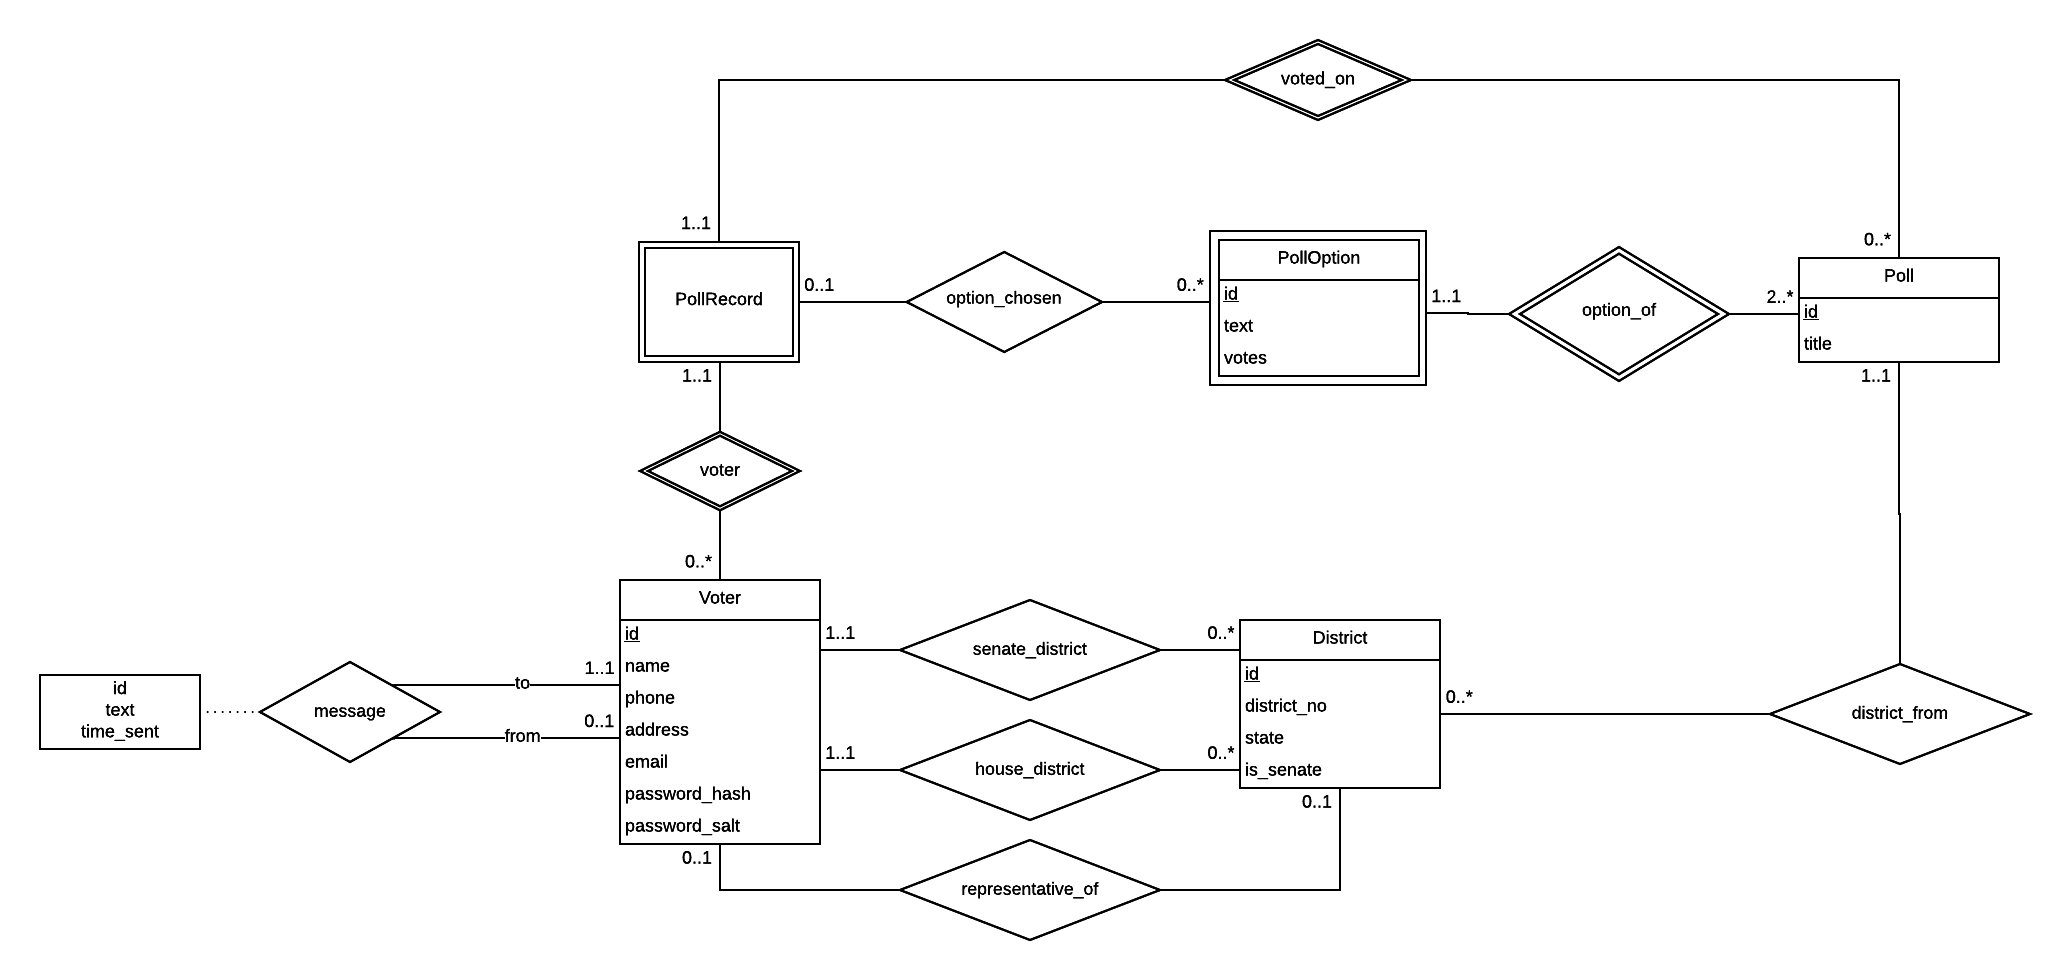
\includegraphics[scale=0.13]{er_diag.png}
\end{figure}
\end{center}
\end{frame}


%
%   Overview
%
\begin{frame}{The Whole Picture}
\begin{itemize}
	\item \textbf{Voters} can possibly be a representative of a district
	\item \textbf{Districts} with voters all have a representative
	\item \textbf{Polls}, created by representatives, have at least two options
	\item \textbf{Poll Records} store a user's choice and ensure a single vote from each user
	\item \textbf{Messages} are between two Voters, and can be optionally anonymous
\end{itemize}
\end{frame}


%
%   Relational Algebra
%
\begin{frame}{A Relational Algebra Translation}
\begin{itemize}
	\item \code{Voter(\underline{id}, name, house\_district, senate\_distict, phone, address, email, password\_hash, password\_salt, district\_representing)}
	\item \code{District(\underline{id}, district\_no, state, is\_senate)}
	\item \code{Poll(\underline{id}, district, title)}
	\item \code{PollOption(\underline{id}, poll, text, votes)}
	\item \code{PollRecord(\underline{voter, poll}, chosen)}
	\item \code{Message(\underline{id}, from, to, text, time\_sent)}
\end{itemize}

\blankfootnote{Underline denotes primary key} 
\end{frame}


%
%   Databases
%
\section{Database Analysis}

\begin{frame}{Functional Dependencies}
\begin{itemize}
	\item Is it 3NF?
	\begin{itemize}
		\item Yes, since each relation has only functional dependencies contained within it's primary key, and therefor a superkey of the relation
	\end{itemize}
	\item Is it BCNF?
	\begin{itemize}
		\item The above statement is also a requirement for BCNF, so yes!
	\end{itemize}
\end{itemize}
\end{frame}


%
%   Sample Query
%
\begin{frame}[fragile]{Sample SQL Queries on \pollaroid}

\begin{lstlisting}[language=SQL]
select
  poll.*,
  count(poll_record.*) as vote_count,
  (select option
   from poll_option
   where poll_option.poll_id = poll.id
   order by votes desc limit 1) as popular_option
from (poll left join poll_record
    on poll.id = poll_record.poll_id)
where poll.district_id in (?,?)
group by poll.id
order by vote_count desc
limit ?;
\end{lstlisting}
\end{frame}

\section{Demonstration}


%
%   Demo
%
\begin{frame}{Let's Try it Out!}
\begin{center}
\url{https://pollaroid.club/} 
\end{center}
\end{frame}

\section{Conclusions}


%
%   Summary
%
\begin{frame}{In Summary...}
\begin{itemize}
	\item \pollaroid removes the disconnect between a representative and the voters of their district
	\item The aim is to promote clarity of viewpoint and popular opinion on a district-to-district basis
	\item Please go to our site and respond to some polls!
\end{itemize}
\end{frame}

\begin{frame}{Questions?}
The \pollaroid Team:
\begin{itemize}
	\item Team Leader: Harlan Haskins
	\item Design Engineer: Joshua Robbins
	\item UI Engineer: Stuart Olivera
	\item Test Engineer: Lucas Shadler
\end{itemize}
\end{frame}
\end{document}
